\section{Experimental Results}\label{s:results}

In this section we present some experimental evaluations of the developed privacy\hyp preserving algorithms.
We try to provide a concise view of our experiments, by carefully selected the most descriptive diagrams.

\subsection{Histograms}\label{ss:results-histograms}

Here we present some experimental results regarding the privacy\hyp preserving histogram computations.
In figure \ref{chart:numerical-histogram} we show the scaling in execution time of histograms on  numerical data (Note: both $x$ and $y$ axes are log\hyp scaled).
In figure \ref{chart:categorical-histogram} we exhibit the respective measurements for histograms on categorical data (Note: both $x$ and $y$ axes are log\hyp scaled).


\begin{figure}[H]
\centering
\centerline{
\begin{minipage}{.5\linewidth}
  \centering
  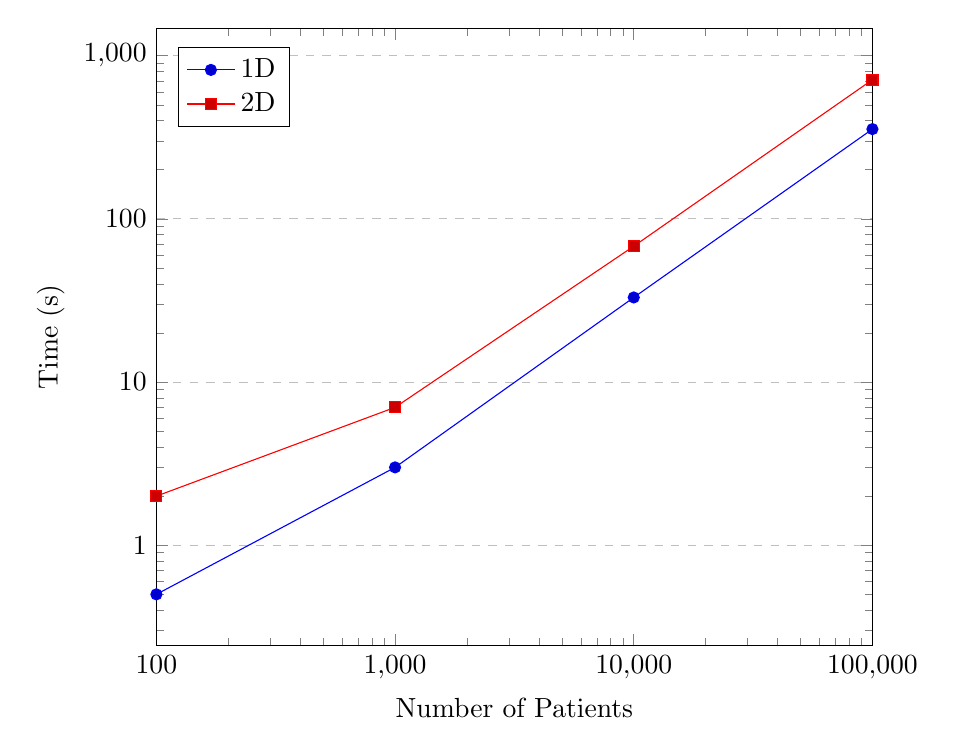
\begin{tikzpicture}
  \begin{axis}[
    legend pos=north west,
    scale only axis,
    enlarge x limits=-1,
    width=\textwidth*0.75,
    ymajorgrids=true,
    xmode=log,
    ymode=log,
    log ticks with fixed point,
    xlabel={Number of Patients},
    ylabel={Time (s)},
    ymin=0,
    grid style=dashed
  ]
  \addplot
    coordinates {(100, 0.5)(1000, 3)(10000, 33)(100000, 355)};
    \addlegendentry{1D}
  \addplot
    coordinates {(100, 2)(1000, 7)(10000, 68)(100000, 713)};
    \addlegendentry{2D}
  \end{axis}
  \end{tikzpicture}
  \caption{Numerical histograms timings}\label{chart:numerical-histogram}
\end{minipage}%
\begin{minipage}{.5\linewidth}
  \centering
  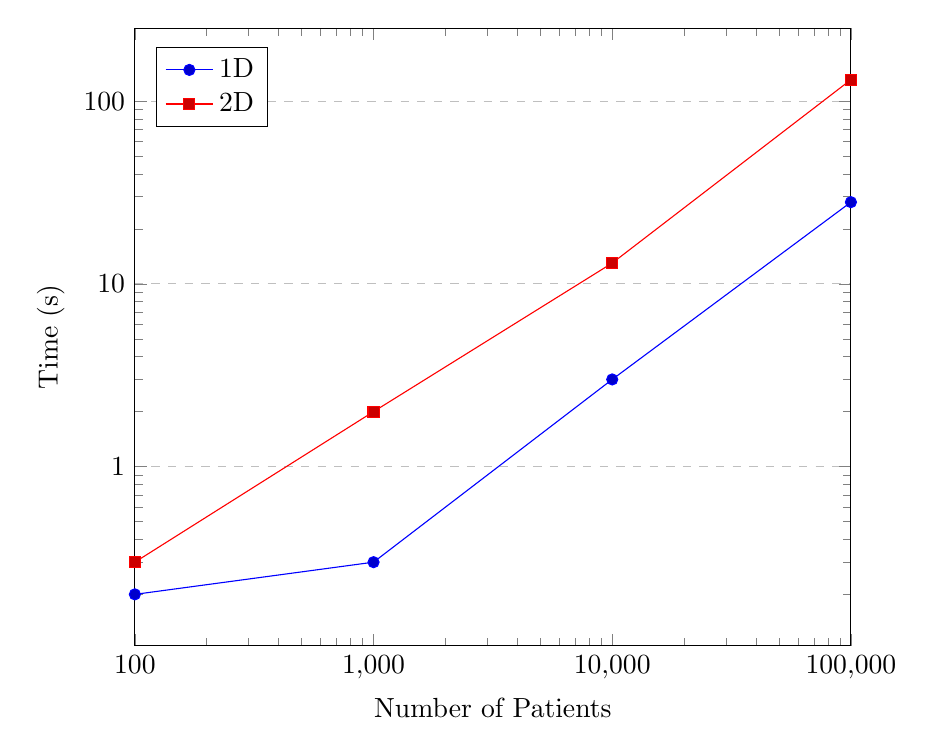
\begin{tikzpicture}
  \begin{axis}[
    legend pos=north west,
    scale only axis,
    enlarge x limits=-1,
    width=\textwidth*0.75,
    ymajorgrids=true,
    xmode=log,
    ymode=log,
    log ticks with fixed point,
    xlabel={Number of Patients},
    ylabel={Time (s)},
    ymin=0,
    grid style=dashed
  ]
  \addplot
    coordinates {(100, 0.2)(1000, 0.3)(10000, 3)(100000, 28)};
    \addlegendentry{1D}
  \addplot
    coordinates {(100, 0.3)(1000, 2)(10000, 13)(100000, 131)};
    \addlegendentry{2D}
  \end{axis}
  \end{tikzpicture}
  \caption{Categorical histograms timings}\label{chart:categorical-histogram}
\end{minipage}
}
\end{figure}

We can see that the histograms on categorical data perform better than their numerical data equivalents especially when applied over bigger datasets.
This is due to the extra computation that needs to be done in the case of numerical data, in order to determine the corresponding histogram cell for each data tuple.
We also see that privacy\hyp preserving histograms are scaling linearly concerning the dataset size, regardless of the type of it.

Below we present the results of similar measurements of histograms on numerical data, but also adding the application of some filters / constraints.
We clearly see that as the dataset grows the number of filters does not make much of a difference in the algorithm's execution time.

%%%%%%%%%%%%%%%%%%%%%%%%%%%%%%%%%%%%%%%%%%%%%%%%%%%%%%%%%%%%%%%%%%%%%%%%%%%%%%%%%%%

\begin{figure}[H]
\centering
\centerline{
\begin{minipage}{.8\linewidth}
  \centering
  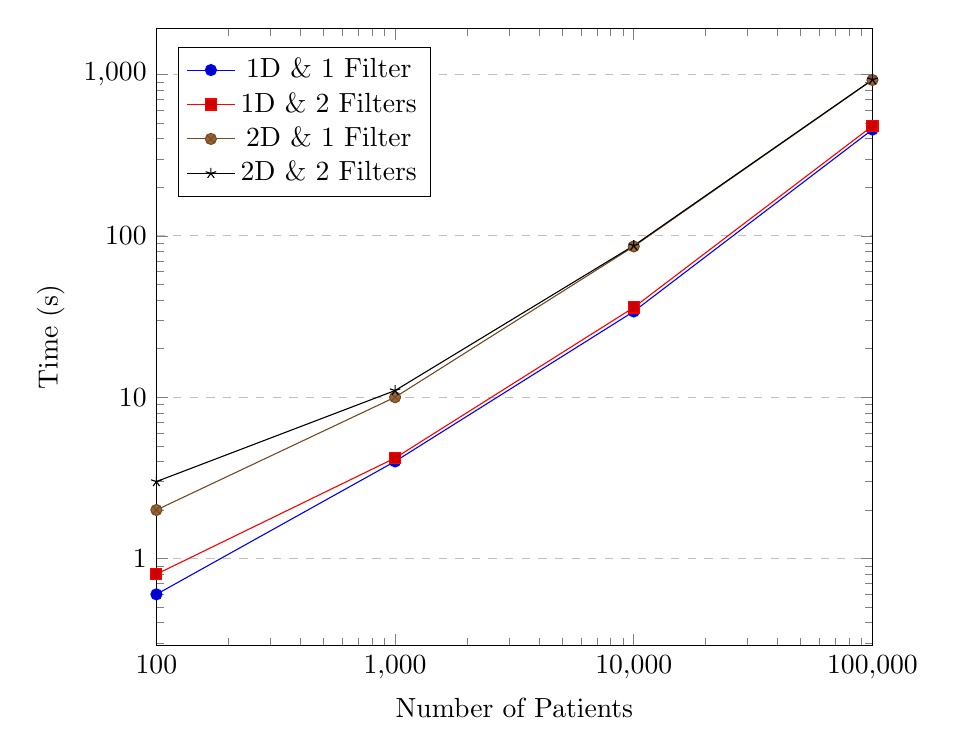
\begin{tikzpicture}
  \begin{axis}[
    legend pos=north west,
    scale only axis,
    enlarge x limits=-1,
    width=\textwidth*0.75,
    ymajorgrids=true,
    xmode=log,
    ymode=log,
    log ticks with fixed point,
    xlabel={Number of Patients},
    ylabel={Time (s)},
    ymin=0,
    grid style=dashed
  ]
  \addplot
    coordinates {(100, 0.6)(1000, 4)(10000, 34)(100000, 456)};
    \addlegendentry{1D \& 1 Filter}
  \addplot
    coordinates {(100, 0.8)(1000, 4.2)(10000, 36)(100000, 480)};
    \addlegendentry{1D \& 2 Filters}
  \addplot
    coordinates {(100, 2)(1000, 10)(10000, 86)(100000, 925)};
    \addlegendentry{2D \& 1 Filter}
  \addplot
    coordinates {(100, 3)(1000, 11)(10000, 87)(100000, 929)};
    \addlegendentry{2D \& 2 Filters}
  \end{axis}
  \end{tikzpicture}
  \caption{Numerical histograms with filters timings}\label{chart:numerical-histogram-filters}
\end{minipage}%
}
\end{figure}


\fixme{Reason (?) about the following chart.}
%%%%%%%%%%%%%%%%%%%%%%%%%%%%%%%%%%%%%%%%%%%%%%%%%%%%%%%%%%%%%%%%%%%%%%%%%%%%%%%%%%%
\begin{figure}[H]
\centering
\centerline{
\begin{minipage}{.8\linewidth}
  \centering
  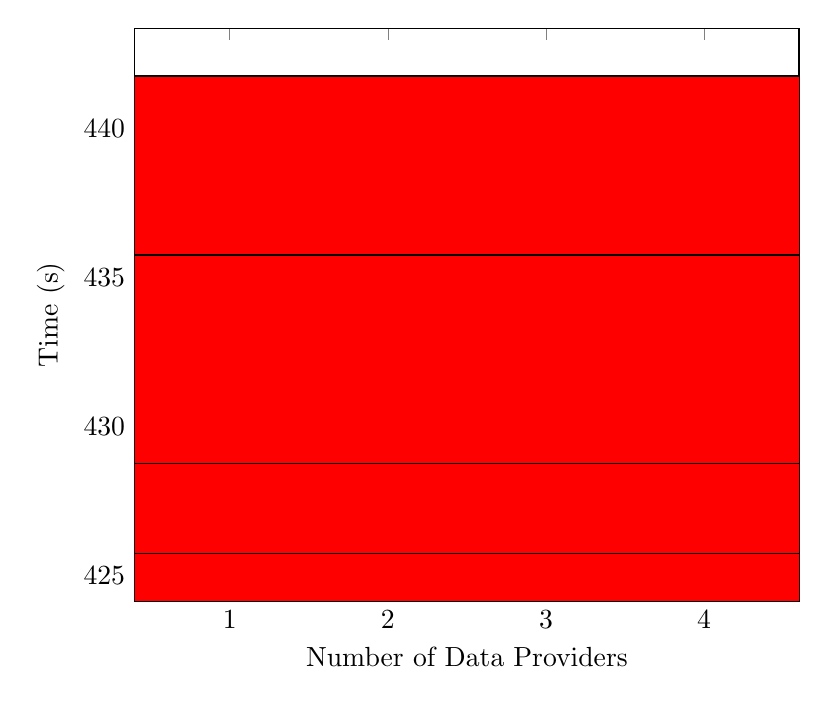
\begin{tikzpicture}
  \begin{axis}[
    legend pos=north west,
    scale only axis,
    ymajorgrids=true,
    xlabel={Number of Data Providers},
    ylabel={Time (s)},
    xtick = {1, 2, 3, 4},
    % ymin = 0,
    grid style=dashed,
    enlarge x limits = 0.2,
    bar width = 40
  ]
  \addplot[ybar, fill=red]
    coordinates {(1, 441.75)(2, 435.75)(3, 428.75)(4, 425.75)};
  \end{axis}
  \end{tikzpicture}
  \caption{Numerical histogram from variable data providers}\label{chart:numerical-histogram-providers}
\end{minipage}%
}
\end{figure}

%%%%%%%%%%%%%%%%%%%%%%%%%%%%%%%%%%%%%%%%%%%%%%%%%%%%%%%%%%%%%%%%%%%%%%%%%%%%%%%%%%%
%%%%%%%%%%%%%%%%%%%%%%%%%%%%%%%%%%%%%%%%%%%%%%%%%%%%%%%%%%%%%%%%%%%%%%%%%%%%%%%%%%%
%%%%%%%%%%%%%%%%%%%%%%%%%%%%%%%%%%%%%%%%%%%%%%%%%%%%%%%%%%%%%%%%%%%%%%%%%%%%%%%%%%%

\subsection{Decision Trees}\label{ss:results-dtrees}

Below you can find time measurements regarding out privacy\hyp preserving classification algorithms.
We have chosen to present results for the ID3 algorithm for the sake of simplicity.
In figure \ref{chart:id3-patients} we show how the algorithm scales as the dataset grows (Note: both $x$ and $y$ axes are log\hyp scaled).
\fixme{Fix y-axis log scaling and ticks}
We have used a fixed number of classification attributes during this measurements.


\begin{figure}[H]
\centering
\centerline{
\begin{minipage}{.8\linewidth}
  \centering
  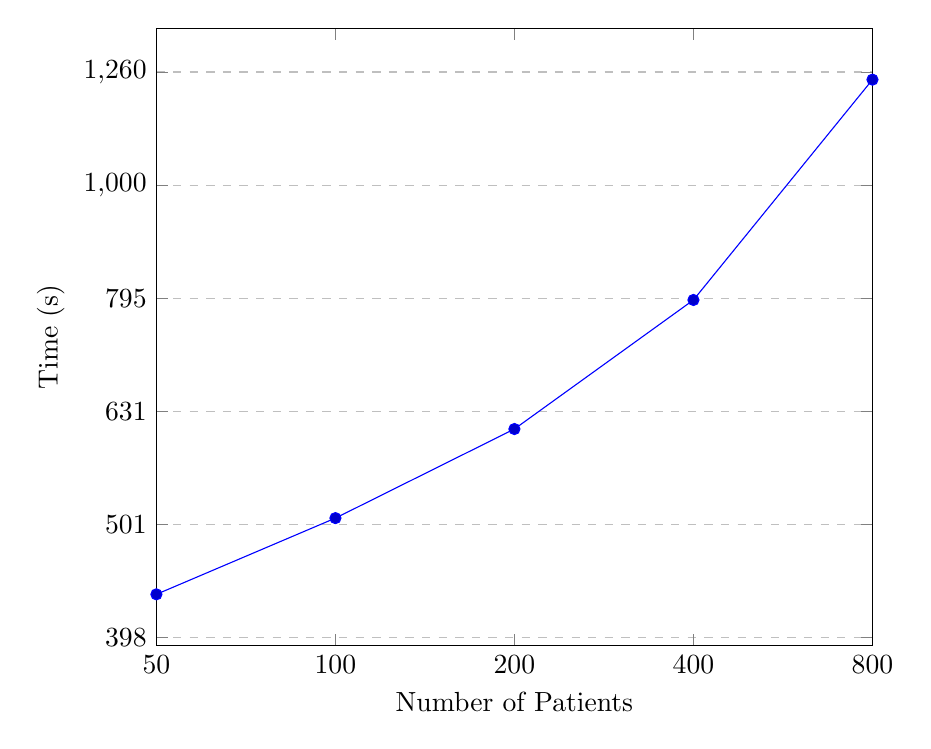
\begin{tikzpicture}
  \begin{axis}[
    legend pos=north west,
    scale only axis,
    enlarge x limits=-1,
    width=\textwidth*0.75,
    ymajorgrids=true,
    xmode=log,
    ymode=log,
    log ticks with fixed point,
    xlabel={Number of Patients},
    xtick = {50, 100, 200, 400, 800},
    ylabel={Time (s)},
    % ymin=0,
    log ticks with fixed point,
    grid style=dashed
  ]
  \addplot
    coordinates {(50, 435)(100, 508)(200, 609)(400, 792)(800, 1240)};
  \end{axis}
  \end{tikzpicture}
  \caption{ID3 decision tree classifier timings with variable patients}\label{chart:id3-patients}
\end{minipage}%
}
\end{figure}

We observe that the execution time of the algorithm is sub\hyp linear regarding the dataset size.
In figure \ref{chart:id3-attributes} you can find the ID3 algorithm timings operating on a constant size dataset, but using variable number of classification attributes.
We can clearly see that the number of attributes used for classification is a dominating factor in the algorithm's performance.

\begin{figure}[H]
\centering
\centerline{
\begin{minipage}{.8\linewidth}
  \centering
  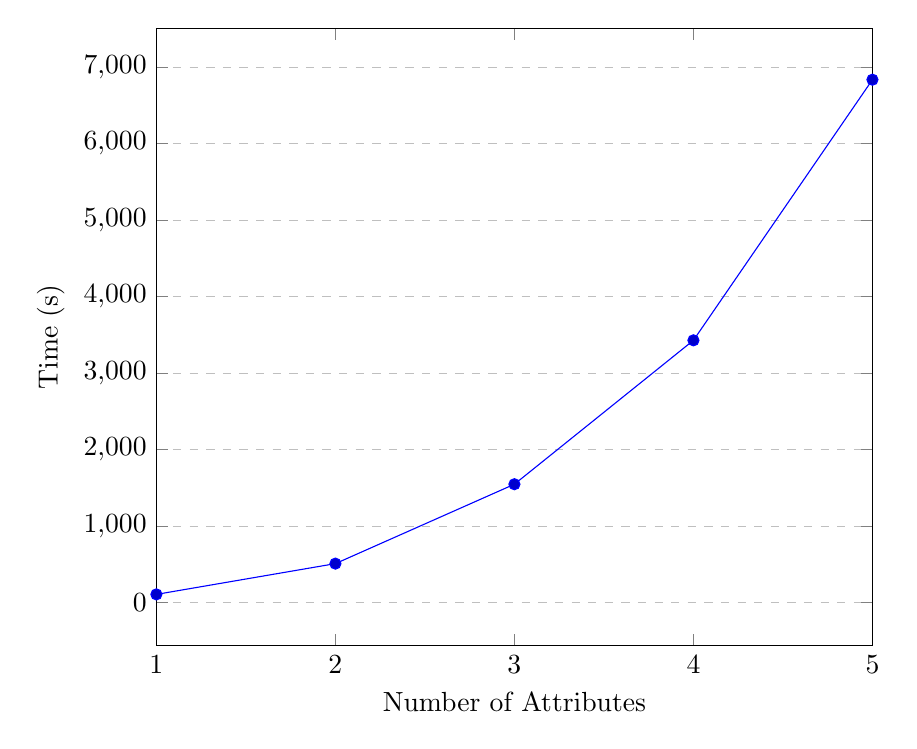
\begin{tikzpicture}
  \begin{axis}[
    legend pos=north west,
    scale only axis,
    enlarge x limits=-1,
    width=\textwidth*0.75,
    ymajorgrids=true,
    log ticks with fixed point,
    xlabel={Number of Attributes},
    xtick = {1, 2, 3, 4, 5},
    ylabel={Time (s)},
    % ymin=0,
    log ticks with fixed point,
    grid style=dashed
  ]
  \addplot
    coordinates {(1, 107)(2, 509)(3, 1547)(4, 3428)(5, 6835)};
  \end{axis}
  \end{tikzpicture}
  \caption{ID3 decision tree classifier timings with variable attributes}\label{chart:id3-attributes}
\end{minipage}%
}
\end{figure}

